\subsection{Loss Functions}\label{subsec:loss-functions}
The main objective of research of loss function is to design such a function which leads to a model with superior
discriminative abilities.
How well the model discriminates can be measured by the compactness of clusters and the distance between them.
The goal is for the clusters to be as compact as possible while maximizing the distance in-between them.

\subsubsection{Softmax Loss}\label{subsubsec:softmax-loss}
Softmax~\cite{ArcFace} is the most widely used loss function in general classification tasks and its definition is as
follows:
\begin{equation}
    \label{eq:softmax}
    \mathcal{L}_S = -\frac{1}{N} \sum_{i=1}^{N} log \frac{e^{W^T_{y_i} x_{i} + b_{y_i}}}
    {\sum_{j-1}^{n} e^{W^T_{j} x_{i} + b_{j}}},
\end{equation}
where $x_i \in \mathbb{R}^{d}$ denotes the feature vector of the \textit{i}-th sample belonging to the $y_i$-th class.
$W_j \in \mathbb{R}^{d}$ is the \textit{j}-th column of the weight matrix $W \in \mathbb{R}^{d \times n}$ and \textit{b}
is the corresponding bias term.
\textit{N} is the batch size and \textit{n} is the class number.

Major drawback of softmax loss is that it doesn't encourage cluster compactness.
In other words, it fails to guarantee similarity among samples within a category.
This makes the learned features not discriminative enough for the open-set face recognition
problem~\footnote{Identifying samples which were not present in the training dataset.}.

The second issue is that the dimension of the output weight matrix grows linearly with the number of identities in the
training set.
This is impractical for large scale deployment.

\subsubsection{Triplet Loss}\label{subsubsec:triplet-loss}
Triplet loss~\cite{TripletLoss} is a loss function which can be optimized by minimizing the distance between
\textit{anchor} and \textit{positive} point while maximizing the distance between \textit{anchor} and \textit{negative}
point.
These points are represented by feature vectors.
The learning process is illustrated in the figure~\ref{fig:tripletloss}.

\begin{figure}[H]
    \centering
    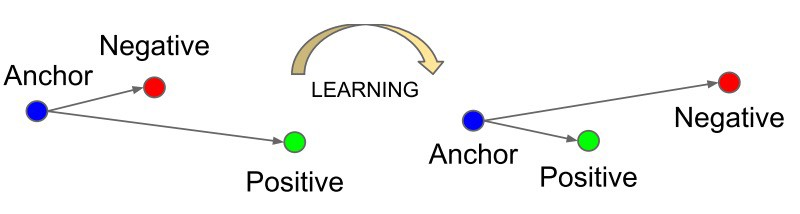
\includegraphics[width=\columnwidth]{images/face-recognition/tripletloss.jpeg}
    \caption{Illustration of the triplet loss~\cite{TripletLoss}}
    \label{fig:tripletloss}
\end{figure}

Anchor and positive points are vectors which belong to the same class whereas negative point belongs to another one.
In the context of facial recognition one class is one identity therefore anchor and positive point are vectorised
representation of two images of one face.

In mathematical terms the loss can be described using Euclidean distance function as follows
\begin{equation}
    \sum_{i}^{N} \left[ \norm{f(x_{i}^{a}) - f(x_{i}^{p}))}^2_2
    - \norm{f(x_{i}^{a}) - f(x_{i}^{n}))}^2_2 + \alpha \right],
\end{equation}
where $f(x_{i}^{a})$, $f(x_{i}^{p})$ and $f(x_{i}^{n})$ are feature vectors of anchor, positive and
negative point of triplet denoted by \textit{i}.
\textit{N} is the number of triplets in the dataset.

The drawbacks of \textit{triplet loss} are the demands entailed by the construction of the triplets.
The number of those is subject to combinatorial explosion and inevitably results in slow convergence and instability
This is a serious issue especially for large datasets.

\subsubsection{Center Loss}
The main objective of the research~\cite{CenterLoss} was to design a loss function which solves the main drawbacks of
\textit{sofmax loss}~\ref{subsubsec:softmax-loss} and \textit{triplet loss}~\ref{subsubsec:triplet-loss}.

The discriminative power of the learned features is enhanced by incorporation of the distance of features to the
corresponding class centers.
In other words, the network is penalized whenever the features are too far from the class center.
In the course of training the the centers are updated and the distances of features from centers are minimized.
The model is trained under a joint supervision of softmax loss and center loss.
The effect of these two losses is balanced by a hyperparameter\footnote{A parameter which is not a subject to the
learning process}.
This joint supervision results in a loss function which combines the best of both worlds:
inter-class discriminative power of \textit{softmax loss} and intra-class distance minimization of \textit{center loss}.

The center loss function is intuitively defined by the following equation:
\begin{equation}
    \label{eq:center}
    \mathcal{L}_C = \frac{1}{2} \sum_{i=1}^{m} \norm{x_i - c_{y_i}}_2^2,
\end{equation}
where $c_{y_i} \in \mathbb{R}^{d}$ denotes the $y_i$-th class center of the features.
Recomputing the centers by taking the average of the features over the whole training set id too inefficient and
impractical.

To address this problem the authors proposed updating the centers based on a mini-batch instead of the whole training
set.
To avoid large perturbations caused by mislabeled samples, there is a parameter $\alpha$ with which we control the
learning rate of the centers.

In the equation~\ref{eq:centup} we can see how the center update is computed:
\begin{align}
    \frac{\partial \mathcal{L}_C}{\partial x_i} &= x_i - c_{y_i} \\
    \Delta c_j &= \frac{\sum_{i=1}^m \delta(y_i=j) \cdot (c_j-x_i)}{1+\sum_{i=1}^m \delta(y_i=j)}, \label{eq:centup}
\end{align}
where $\delta(condition)$ is $1$ if the condition is satisfied and $0$ otherwise.

The final loss is described by the following formula:
\begin{equation}
    \label{eq:centerloss}
    \mathcal{L} = \mathcal{L}_S + \mathcal{L}_C = -\sum_{i=1}^{m} log \frac{e^{W^T_{y_i} x_{i} + b_{y_i}}}
    {\sum_{j-1}^{n} e^{W^T_{j} x_{i} + b_{j}}} + \frac{\lambda}{2} \sum_{i=1}^{m} \norm{x_i - c_{y_i}}_2^2,
\end{equation}

Figure~\ref{fig:centerlosslambda} is a great visualization of the effect of hyperparameter $\alpha$ upon the cluster
compactness.
As is to be expected, higher values of the parameter result in more compact clusters.

\begin{figure}[H]
    \centering
    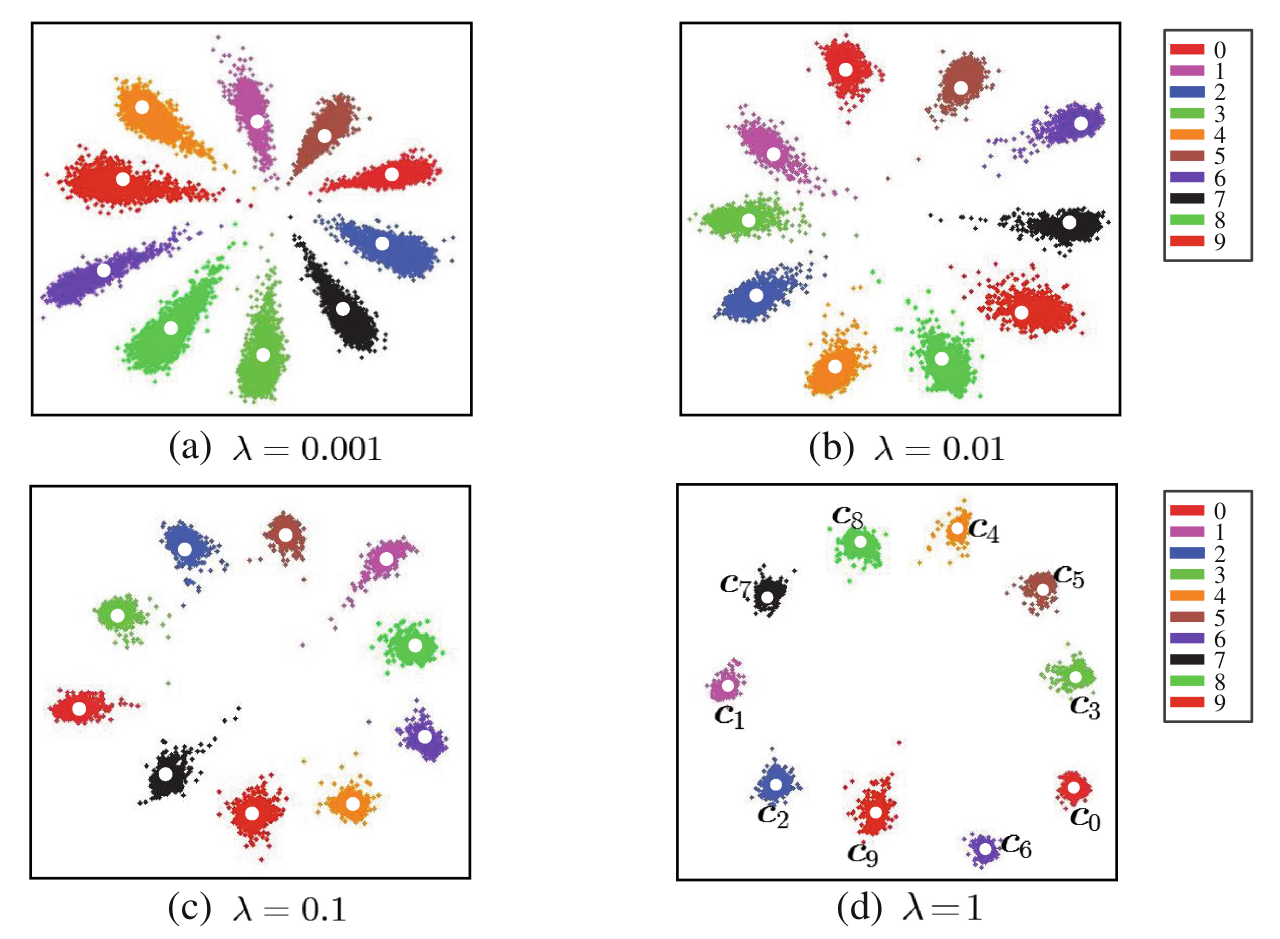
\includegraphics[width=\columnwidth]{images/face-recognition/centerlosslambda.png}
    \caption{Distribution of the features for different values of hyperparameter $\lambda$~\cite{CenterLoss}.
    The white dots $(c_0,c_1,\dots,c_9)$ denote 10 class centers.}
    \label{fig:centerlosslambda}
\end{figure}

\subsubsection{Congenerous Cosine Loss}
Congenerous Cosine Loss~\cite{CocoLoss} (known as COCO loss) is a loss function which was published in 2017.

To define the loss we first have to clarify how the centroid of class \textit{k} is computed.
The centroid\footnote{Center of cluster.} equation is as follows
\begin{equation}
    \boldsymbol{c}_{k} = \frac{\sum_{i \in \beta} \delta \left( l_i, k \right)\boldsymbol{f}^{(i)}}
    {\sum_{i \in \beta} \delta \left( l_i, k \right) + \epsilon} \in \mathbb{R}^{D \times 1},
\end{equation}
where $\beta$ is a mini-batch, $D$ is the feature space dimension, $\delta$ is indicator function, $\epsilon$ is a
trivial number for computation stability, $\boldsymbol{f}^{(i)}$ is the \textit{i}-th feature vector and $l_i$ is
its label.

Now that we have the centroid equation we can define the term we are trying to maximize during model fitting:
\begin{equation}
    p_{l_i}^{(i)} = \frac{exp C(\boldsymbol{f}^{(i)}, \boldsymbol{c}_{l_{i}})}
    {\sum_{k \neq l} exp C(\boldsymbol{f}^{(i)}, \boldsymbol{c}_{k})} \in \mathbb{R},
\end{equation}
where $C$ is standard cosine similarity.

Now we can move on to the final COCO loss function definition:
\begin{equation}
    - \sum_{i \in \beta} log \left( p_{l_i}^{(i)} \right).
\end{equation}

\subsubsection{SphereFace Loss}
SphereFace~\cite{SphereFace} is a loss function which was published in 2018.
The research significantly distinguishes itself from the previously mentioned losses by not relying on euclidean margin.
SphereFace uses angular margin instead.
This has proven to be highly effective in face recognition tasks.

SphereFace loss originates from the softmax loss~\ref{subsubsec:softmax-loss} and its name was inspired by the fact
that the features are projected onto a hypersphere manifold.

To derive SphereFace loss from softmax loss we first incorporate the angle into the softmax equation using the dot
product definition ($a \cdot b = \norm{a} \norm{b} cos \theta$):

\begin{align*}
    \mathcal{L}_S &= -\frac{1}{N} \sum_{i=1}^{N} log \frac{e^{W^T_{y_i} x_{i} + b_{y_i}}}
    {\sum_{j-1}^{n} e^{W^T_{j} x_{i} + b_{j}}} \\
    &= -\frac{1}{N} \sum_{i=1}^{N} log \frac{e^{\norm{W_{y_i}} \norm{x_i} cos(\theta_{y_i,i}) + b_{y_i}}}
    {\sum_{j-1}^{n} e^{\norm{W_j} \norm{x_{i}} cos(\theta_{j,i}) + b_{j}}},
\end{align*}
where $\theta_{j,i}$ is the angle between vector $W_j$ and $x_i$.
The meanings of the remaining symbols are equal to those in the softmax equation~\ref{eq:softmax}.


Next we normalize $\norm{W_j} = 1, \forall j$ and set the bias term to 0.
\begin{equation}
    \mathcal{L}_{modified} = -\frac{1}{N} \sum_{i=1}^{N} log \frac{e^{\norm{x_i} cos(\theta_{y_i,i})}}
    {\sum_{j-1}^{n} e^{\norm{x_{i}} cos(\theta_{j,i})}}
\end{equation}
While it's possible to learn features with the modified loss the features are not discriminative enough.
To improve the discriminative power angular margin was incorporated:
\begin{equation}\label{eq:ang}
\mathcal{L}_{ang} = -\frac{1}{N} \sum_{i=1}^{N} log \frac{e^{\norm{x_i} cos(m\theta_{y_i,i})}}
{e^{\norm{x_i} cos(m\theta_{y_i,i})} + \sum_{j \neq y_i} e^{\norm{x_{i}} cos(\theta_{j,i})}},
\end{equation}
where $\theta_{y_i,i}$ lies in $\left[ 0, \frac{\pi}{m} \right]$.

To make the loss~\ref{eq:ang} optimizable for CNNs the definition range of $cos(\theta_{y_i},i)$ is expanded.
This is achieved by replacing the cosine term with monotonically decreasing angle function $\Psi(\theta_{y_i},i)$
\begin{equation}
    \mathcal{L}_{ang} = -\frac{1}{N} \sum_{i=1}^{N} log \frac{e^{\norm{x_i} \Psi(m\theta_{y_i,i})}}
    {e^{\norm{x_i} \Psi(m\theta_{y_i,i})} + \sum_{j \neq y_i} e^{\norm{x_{i}} \Psi(\theta_{j,i})}}
\end{equation}
The angle function has the following definition:
\begin{equation}
    \Psi(\theta_{y_i,i}) = (-1)^{k} cos(\theta_{y_{i},i}) -2k,
\end{equation}
where $k \in \left[ 0, m-1 \right]$.
Parameter $m \geq 1$ gives us the control over the angular margin size.


\subsubsection{ArcFace Loss}\label{subsubsec:arcface}
ArcFace loss is used in this thesis which makes it the topic of the following chapter~\ref{ch:arcface}.